\begin{figure}
    \centering
        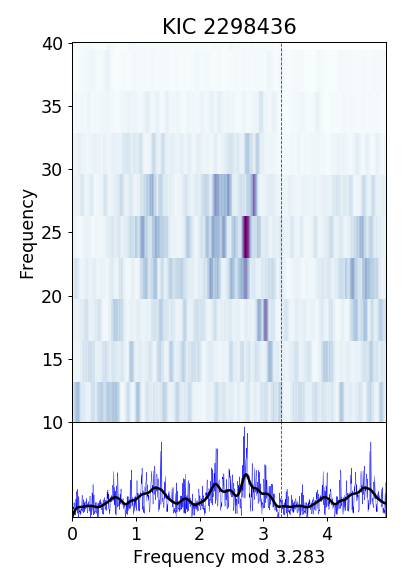
\includegraphics[width=0.3\textwidth]{Chapter5/2298436_echelle.png}
        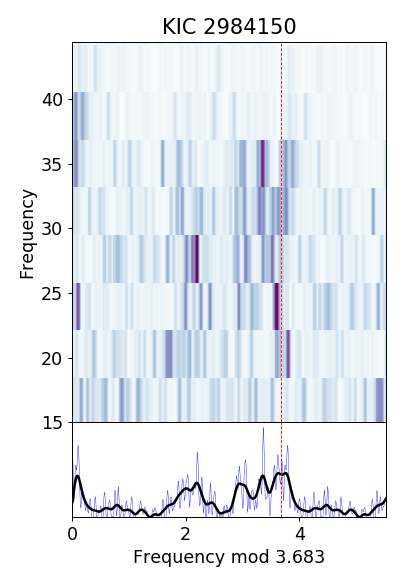
\includegraphics[width=0.3\textwidth]{Chapter5/2984150_echelle.png}
        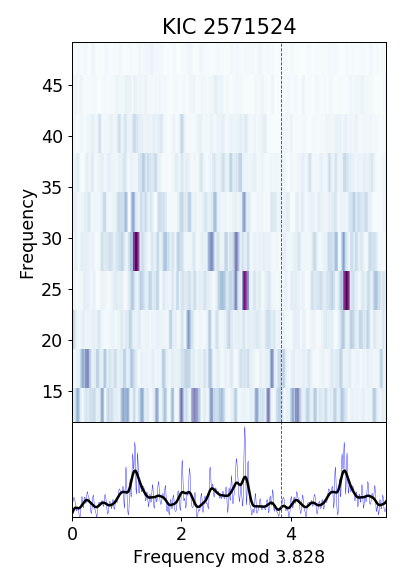
\includegraphics[width=0.3\textwidth]{Chapter5/2571524_echelle.png}
        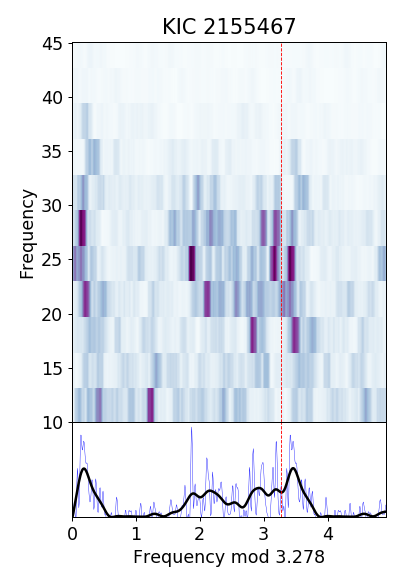
\includegraphics[width=0.3\textwidth]{Chapter5/2155467_echelle.png}
        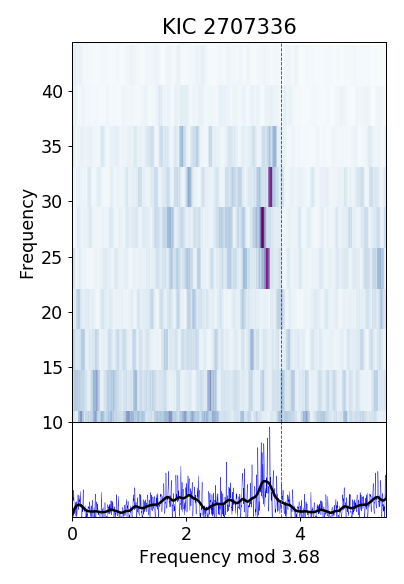
\includegraphics[width=0.3\textwidth]{Chapter5/2707336_echelle.png}
    \caption[\'Echelle diagrams for the newly identified cluster red giants in NGC\,6791 (I)]{\'Echelle diagrams for the newly identified NGC\,6791 red giants, ordered by \numax{}. The red line represents \dnu{} with the \'echelle extended to 1.5 \dnu{} to aid in identifying the $l = 0$ modes when $\epsilon$ is around 1.}
    \label{fig:echelle_new_6791}
\end{figure}

\begin{figure}
    \centering
        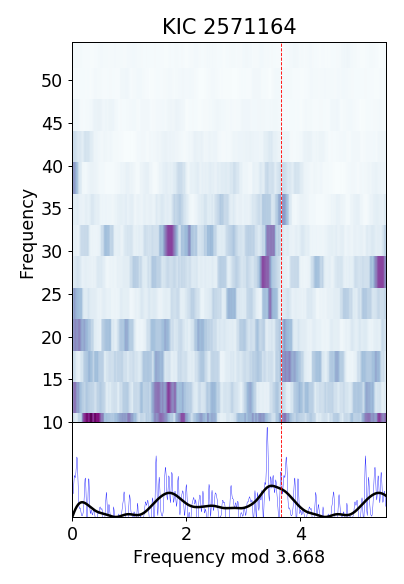
\includegraphics[width=0.3\textwidth]{Chapter5/2571164_echelle.png}
        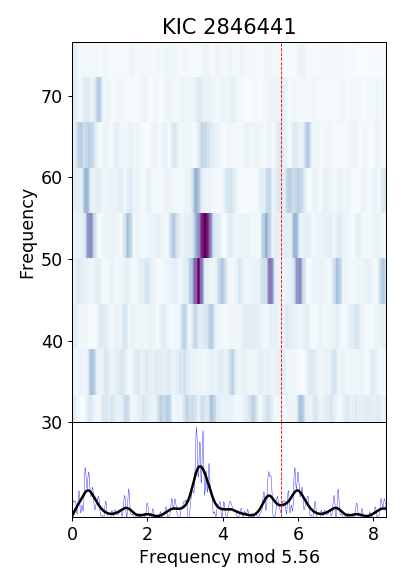
\includegraphics[width=0.3\textwidth]{Chapter5/2846441_echelle.png}
        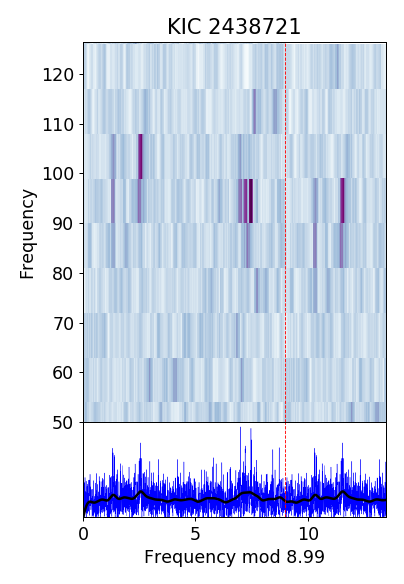
\includegraphics[width=0.3\textwidth]{Chapter5/2438721_echelle.png}
        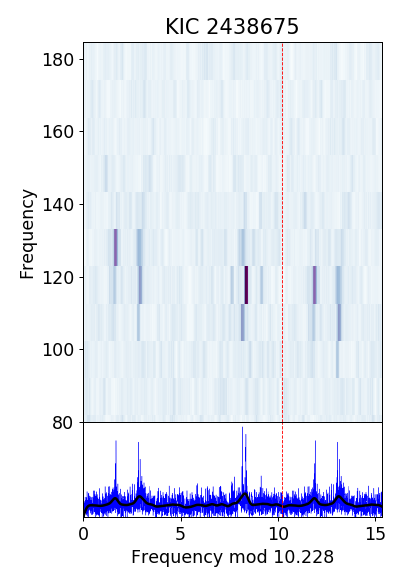
\includegraphics[width=0.3\textwidth]{Chapter5/2438675_echelle.png}
        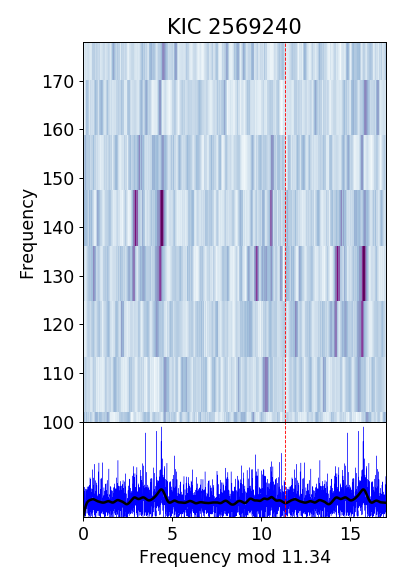
\includegraphics[width=0.3\textwidth]{Chapter5/2569240_echelle.png}
    \caption[\'Echelle diagrams for the newly identified cluster red giants in NGC\,6791 (II)]{Continued from Figure \ref{fig:echelle_new_6791}}
    \label{fig:echelle_new2_6791}
\end{figure}

\begin{figure}
    \centering
        % 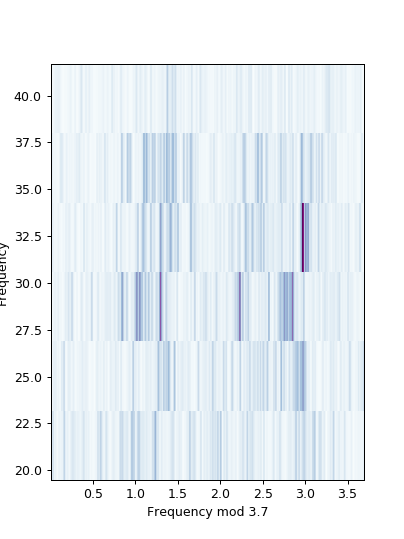
\includegraphics[width=0.32\textwidth]{Chapter5/2437817_echelle_new.png}
        % 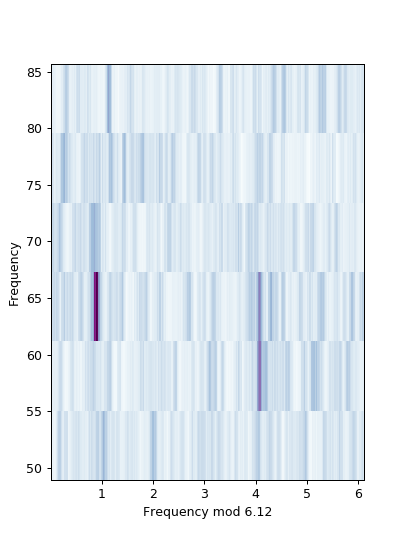
\includegraphics[width=0.32\textwidth]{Chapter5/2438053_echelle_new.png}
        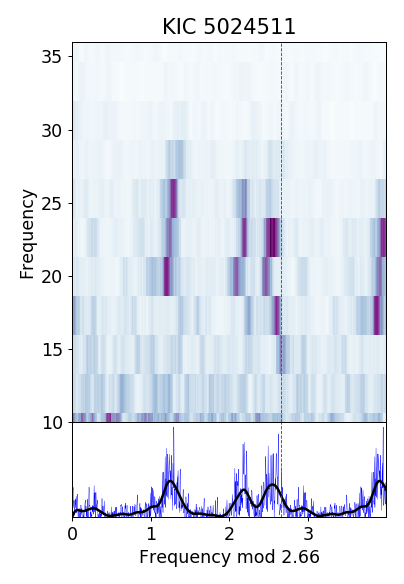
\includegraphics[width=0.32\textwidth]{Chapter5/5024511_echelle.png}
        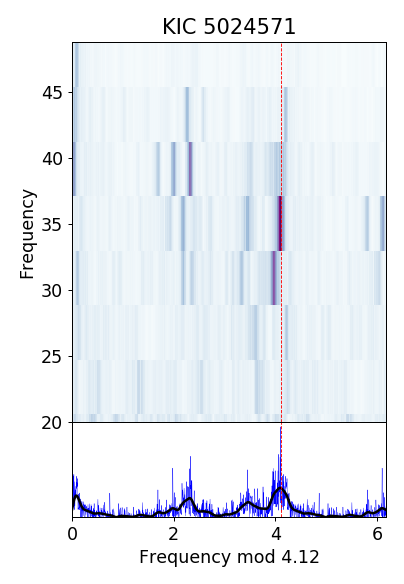
\includegraphics[width=0.32\textwidth]{Chapter5/5024571_echelle.png}
        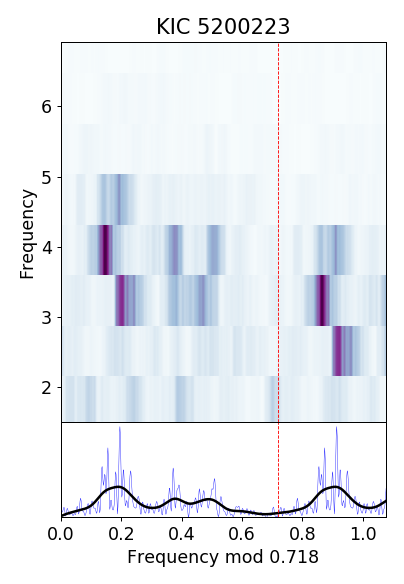
\includegraphics[width=0.32\textwidth]{Chapter5/5200223_echelle.png}
        % 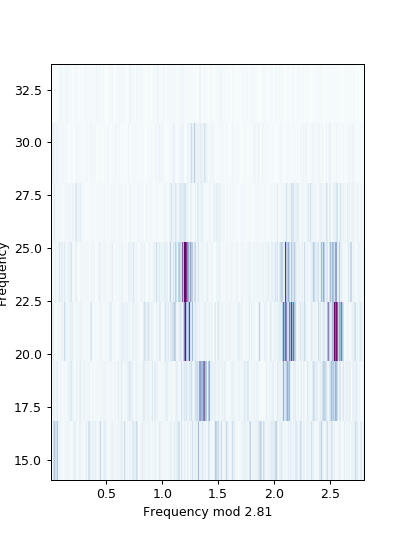
\includegraphics[width=0.32\textwidth]{Chapter5/5025060_echelle_new.png}
    \caption[\'Echelle diagrams for the newly identified cluster red giants in NGC\,6819 (I)]{Same as Figure \ref{fig:echelle_new_6791} but for NGC\,6819.}
    \label{fig:echelle_new_6819}
\end{figure}

\begin{figure}
    \centering
    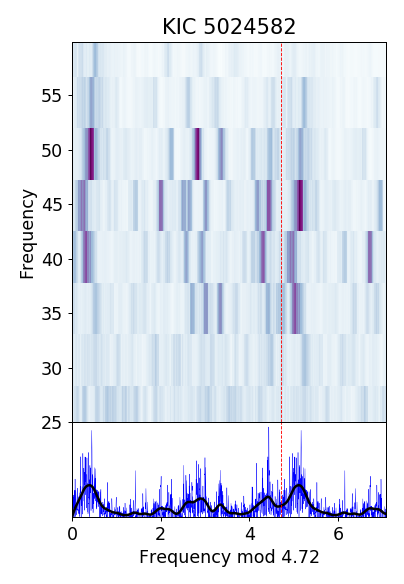
\includegraphics[width=0.32\textwidth]{Chapter5/5024582_echelle.png}
    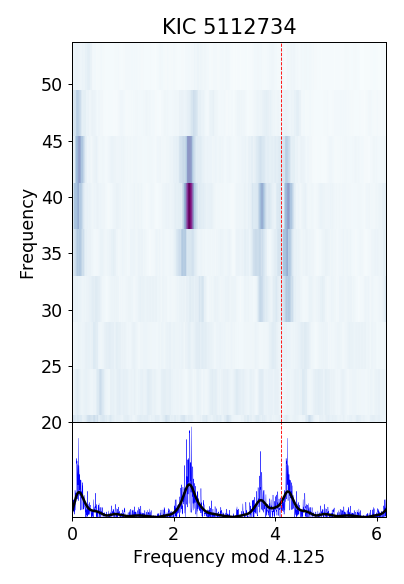
\includegraphics[width=0.32\textwidth]{Chapter5/5112734_echelle.png}
    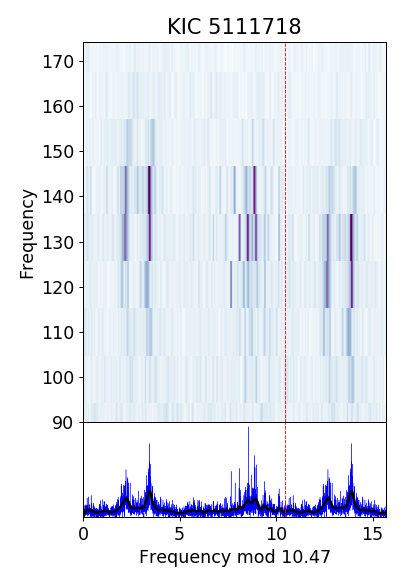
\includegraphics[width=0.32\textwidth]{Chapter5/5111718_echelle.png}
    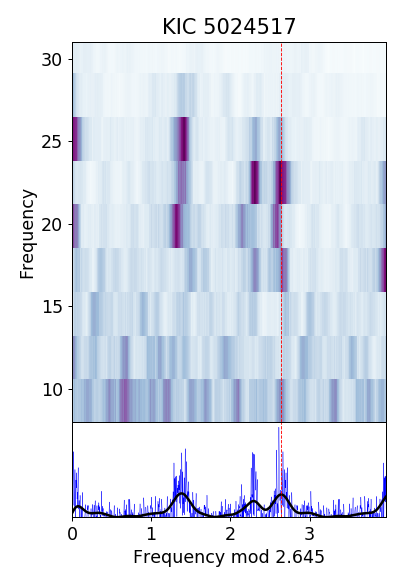
\includegraphics[width=0.32\textwidth]{Chapter5/5024517_a_echelle.png}
    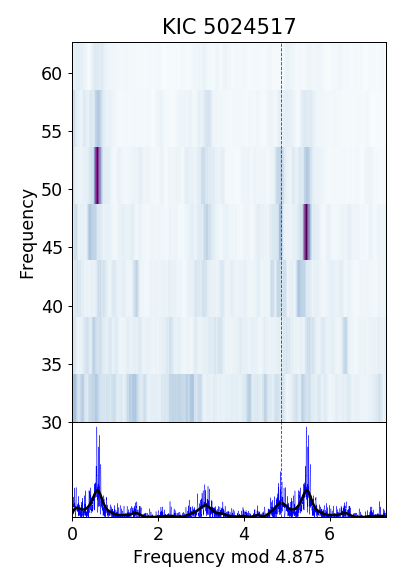
\includegraphics[width=0.32\textwidth]{Chapter5/5024517_b_echelle.png}
    
    \caption[\'Echelle diagrams for the identified cluster red giants in NGC\,6819 (II)]{Same as Figure \ref{fig:echelle_new_6819} for stars identified in Beau's thesis \citep{bellamy_using_2015}, that we have produced \`echelle diagrams for, for the first time. The last two panels show individual \`echelle diagrams for the two red giant power excesses we have identified in KIC\,5024517.}
    \label{fig:echelle_new2_6819}
\end{figure}